\chapter{Introduction}
\label{chap:introduction}
# TODO: DIese Struktur in intro einbauen ohne diese Soprachorgasmen
\section{Initial Situation}
The dawn of the fourth industrial revolution, commonly known as Industry 4.0, has ushered in an era of unprecedented technological transformation. This revolution is characterized by the convergence of cyber-physical systems (CPS), the Internet of Things (IoT), and cloud computing, collectively creating the foundation for smart factories driven by automation and efficiency \parencite{Oztemel2020}. Within this evolving industrial landscape, companies strive to remain competitive by embracing innovative technologies that promise enhanced productivity and reduced operational costs.
Among these transformative technologies, the Digital Twin (DT) has emerged as a particularly powerful concept. A Digital Twin can be defined as a virtual representation of physical assets that enables real-time monitoring and optimization \parencite{Tao2018ijamt}. More than a simple simulation, it serves as an enabling technology that bridges the physical and digital realms through bi-directional data flow, allowing for information exchange and influencing the behavior of physical assets \parencite{grieves2014digital}. This seamless connection facilitates real-time data integration, simulation, and optimization, embodying the core promise of Industry 4.0 \parencite{judijanto2024trends}.
Although this field is rapidly evolving, consensus on the precise definition of Digital Twins remains elusive. The term was first introduced by Michael Grieves in 2002, initially defined as a digital representation of a physical object or system \parencite{grieves2014digital}. Since then, the concept has expanded considerably, encompassing a broader range of applications and technologies. Throughout the literature, three related but distinct terms have emerged to describe similar characteristics: Digital Model (DM), Digital Shadow (DS), and Digital Twin (DT) \parencite{jones2020characterising,Zhang2021jmsy}.
\begin{figure}[htbp]
  \centering
  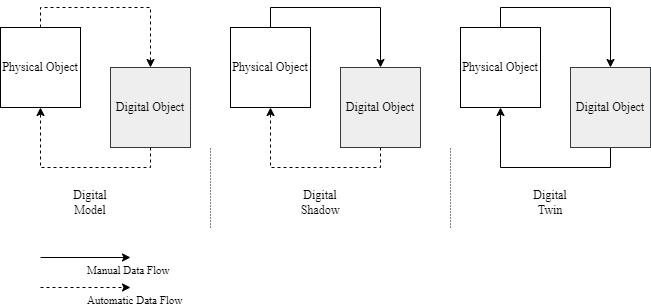
\includegraphics[width=0.8\textwidth]{figures/kritzinger.png}
  \caption{Comparison of Digital Shadow (DS), Digital Model (DM) and Digital Twin (DT) as presented by Kritzinger. This distinction is crucial for understanding validation requirements across different digital representation types.}
  \label{fig:Kritzinger}
\end{figure}
The Digital Model represents the most basic form, containing only manual data connections between physical and digital entities. These connections can be temporarily shifted or disconnected, and the digital object exercises no control over the physical entity. The Digital Model serves purely descriptive purposes, unable to make autonomous decisions or influence the physical object, with control remaining entirely in the hands of the modeller.
A step further in sophistication, the Digital Shadow continuously updates with real-time data from its physical counterpart. While more advanced than a Digital Model, it remains limited to monitoring, analysis, and simulation, predicting future states based on current and historical data but lacking the ability to influence the physical object. Similar to the Digital Model, control remains with the modeller, though Digital Shadows are frequently—and sometimes confusingly—classified as Digital Twins in literature.
The true Digital Twin represents the pinnacle of these technologies. Like the Digital Shadow, it receives continuous real-time updates, but crucially, it can also send control signals to influence the physical object. This bidirectional relationship enables the Digital Twin to serve purposes beyond modeling and simulation, potentially functioning as an autonomic system that updates itself or operates with minimal modeller intervention \parencite{kritzinger2018digital}.
The adoption of Digital Twins spans numerous sectors, with \cite{jeremiah2024comprehensive} identifying urban planning, robotics, manufacturing, aviation, healthcare, and system engineering as primary application areas. The greatest concentration of Digital Twin developments occurs in urban and manufacturing environments \parencite{sanabria}, with various creation methodologies detailed by \cite{schwede2024learning}.

Despite their transformative potential, implementing Digital Twins entails significant challenges. The creation and maintenance of accurate Digital Twins require substantial investment in both technology and expertise. This investment yields no return if the resulting model fails to accurately represent the modelled entity or delivers incorrect results. As industries integrate Digital Twins into their production processes, establishing trust becomes fundamental \parencite{trauer2022digital}. To gain widespread acceptance, the technology must demonstrate accuracy, transparency, and cost-efficiency \parencite{Wright2020amse}. Without these qualities, organizations will likely default to familiar methods, potentially fostering resistance to technological advancement.
To address these adoption barriers, several strategies have emerged. One approach focuses on enhancing the intrinsic explainability of Digital Twins, reducing their black-box characteristics through improved visualizations, explanations, communication channels, and transparency \parencite{arrieta2020explainable}. Another critical strategy involves ensuring the validity, reliability, and accuracy of the Digital Twin through rigorous validation and verification (V&V) processes.
Validation and verification represent essential quality assurance methodologies in modeling and simulation. Validation assesses whether a Digital Twin accurately represents its physical counterpart for its intended purpose, while verification confirms that the computational implementation correctly reflects the conceptual model. Before advancing toward "responsible" AI integration \parencite{dwivedi2023explainable}, Digital Twins must undergo expert-led V&V processes to establish their reliability. As \cite{Shao2023mfglet} and \cite{Wright2020amse} emphasize, these approaches are vital for building trust and credibility.
The considerable expense associated with creating Digital Twins has driven interest in automated generation methods, particularly those leveraging existing operational data. These approaches promise to reduce both development costs and time-to-implementation. However, this automation introduces new challenges for validation and verification. Traditional V&V approaches typically require case-specific reference values and substantial manual expert involvement—requirements that conflict with the efficiency goals of automated twin generation.
For discrete material flow systems, these challenges intensify due to the dynamic nature of operations and inherent stochastic elements. When Digital Twins for these systems are generated automatically, conventional validation approaches become particularly problematic, as they negate much of the efficiency gained through automation.
This creates an apparent paradox: automated Digital Twin generation reduces initial development effort but potentially increases subsequent validation complexity. This thesis addresses this paradox by proposing that object-centric event logs—the same data structures often used to generate these twins—can serve as the foundation for an automated, use case-independent validation and verification framework. Such an approach would maintain the efficiency benefits of automated generation while ensuring the resulting Digital Twins meet necessary quality standards.

\section{Problem}
% Content goes here

\section{Objective of the Thesis}
% This section includes: Motivation, Relevance, Research Questions, and Hypotheses
% Content goes here

\section{Structure of the Thesis and Methodological Approach}
% Content goes here

\chapter{Introduction}

Diese Arbeit befasst sich mit der automatisierten Verifikation und Validierung von automatisiert generierten, simulationsbasierten digitalen Zwillingen für diskrete Materialflusssysteme. Im Zuge der Digitalisierung industrieller Prozesse und der vierter industriellen Revolution (Industrie 4.0) gewinnen digitale Zwillinge zunehmend an Bedeutung. Die vorliegende Einleitung skizziert zunächst die aktuelle Situation und den daraus resultierenden Bedarf, formuliert das zentrale Problem sowie die Zielsetzung der Arbeit und erläutert abschließend den Aufbau sowie die methodische Vorgehensweise.

\section{Initial Situation}

Im Rahmen der vierten industriellen Revolution findet eine verstärkte Integration von Informations- und Kommunikationstechnologien in Produktions- und Logistikprozesse statt. Digitale Zwillinge, also virtuelle Repliken physischer Systeme, ermöglichen nicht nur die Überwachung von Anlagen, sondern auch deren dynamische Simulation und Optimierung. Besonders in diskreten Materialflusssystemen – wie sie in der Automobilindustrie, der Logistik oder in hochautomatisierten Fertigungsprozessen vorkommen – erweist sich die präzise Modellierung von Materialflüssen als Schlüsselfaktor für Effizienz und Wettbewerbsfähigkeit \parencite{Grieves2014}.

Die rasante Entwicklung im Bereich der Sensorik und des Internet of Things (IoT) liefert kontinuierlich große Datenmengen, die in digitalen Zwillingen genutzt werden können, um den aktuellen Zustand von Produktionssystemen nahezu in Echtzeit abzubilden. Traditionelle Simulationsansätze, die oft auf statischen Modellen basieren, werden durch die dynamische Natur digitaler Zwillinge ergänzt, die durch kontinuierliche Datenintegration eine verbesserte Prozesssteuerung und prädiktive Instandhaltung ermöglichen \parencite{Tao2018}. Dabei stellen digitale Zwillinge eine Schnittstelle zwischen der realen und der virtuellen Welt dar und bieten somit die Möglichkeit, komplexe industrielle Abläufe zu überwachen, zu simulieren und zu optimieren.

Die zunehmende Digitalisierung und Vernetzung führen jedoch auch zu neuen Herausforderungen. Die Komplexität moderner Systeme sowie die enorme Datenflut erfordern innovative Ansätze zur Modellierung und kontinuierlichen Aktualisierung. Hierbei steht insbesondere die automatisierte Generierung von Simulationsmodellen im Vordergrund, die durch datengetriebene Verfahren unterstützt wird. Dieser Paradigmenwechsel fordert nicht nur traditionelle Simulationsmethoden heraus, sondern eröffnet auch neue Perspektiven für die industrielle Praxis, indem er die Grundlage für eine optimierte Entscheidungsfindung schafft \parencite{Uhlemann2017}.

\section{Problem}

Trotz des hohen Potenzials digitaler Zwillinge treten in der Praxis zahlreiche Herausforderungen auf. Die automatisierte Erstellung simulationsbasierter Modelle birgt das Risiko, dass wesentliche Systemkomponenten oder Interaktionsmuster unzureichend erfasst werden. Dies führt zu Diskrepanzen zwischen dem digitalen Modell und dem realen System, was im schlimmsten Fall die Grundlage für fehlerhafte Simulationen und falsche betriebliche Entscheidungen bildet. Traditionelle Verifikations- und Validierungsprozesse (V\&V) basieren häufig auf manuellen Prüfungen, die angesichts der Komplexität und der Datenmengen in modernen Produktionssystemen nicht mehr effizient durchführbar sind \parencite{Kritzinger2018}.

Ein weiteres Problemfeld stellt die Integration von Echtzeitdaten in die Simulationsmodelle dar. Während historische Daten die Basis statischer Modelle bilden, erfordert die dynamische Anpassung digitaler Zwillinge die kontinuierliche Auswertung und Synchronisation aktueller Betriebsdaten. Dies führt zu Herausforderungen hinsichtlich der Datenkonsistenz, -qualität und -verarbeitung. Zudem fehlt es oft an standardisierten Bewertungsmetriken, die eine objektive Beurteilung der Modellgüte ermöglichen. Diese Probleme machen deutlich, dass herkömmliche V\&V-Methoden nicht ohne Weiteres auf automatisiert generierte, simulationsbasierte digitale Zwillinge übertragbar sind.

Insbesondere in diskreten Materialflusssystemen, in denen zahlreiche Prozessvariablen und Interaktionskomponenten eine Rolle spielen, erfordert die Sicherstellung der Modellgenauigkeit neue Ansätze. Es besteht daher dringender Forschungsbedarf, um datengetriebene und automatisierte V\&V-Methoden zu entwickeln, die den spezifischen Anforderungen solcher Systeme gerecht werden \parencite{Kritzinger2018, Uhlemann2017}.

\section{Objective of the Thesis}

Das Hauptziel dieser Arbeit ist die Entwicklung eines datengetriebenen Frameworks zur automatisierten Verifikation und Validierung von digital generierten, simulationsbasierten digitalen Zwillingen. Der Fokus liegt dabei auf diskreten Materialflusssystemen, da diese aufgrund ihrer Komplexität und Dynamik besondere Herausforderungen hinsichtlich der Modellgenauigkeit und Prozesssynchronisation aufweisen.

\subsection*{Motivation und Relevanz}

Die Motivation dieser Forschungsarbeit ergibt sich aus mehreren zentralen Aspekten:
\begin{itemize}
  \item \textbf{Effizienzsteigerung:} Durch den Einsatz automatisierter V\&V-Methoden können Modellabweichungen frühzeitig erkannt und behoben werden, was zu einer signifikanten Reduktion von Fehlerquellen und Optimierungspotenzialen in Produktionsprozessen führt.
  \item \textbf{Digitalisierung und Vernetzung:} Mit der zunehmenden Integration von IoT und Sensorik in Produktionsanlagen steigt die Verfügbarkeit von Echtzeitdaten, die in digitalen Zwillingen verarbeitet werden können. Ein zuverlässiges V\&V-Framework stellt sicher, dass diese Daten adäquat in die Modelle einfließen.
  \item \textbf{Wettbewerbsvorteile:} Unternehmen, die in der Lage sind, ihre digitalen Modelle präzise und effizient zu validieren, sichern sich langfristig Wettbewerbsvorteile in einem zunehmend globalisierten Marktumfeld \parencite{Grieves2014}.
\end{itemize}

\subsection*{Forschungsfragen und Hypothesen}

Die Arbeit fokussiert sich auf folgende Forschungsfragen:
\begin{itemize}
  \item Wie können automatisierte Prozesse zur Verifikation und Validierung von digital generierten, simulationsbasierten digitalen Zwillingen effizient implementiert werden?
  \item Welche datengetriebenen Ansätze eignen sich am besten, um Abweichungen zwischen simuliertem Verhalten und realen Betriebsdaten in diskreten Materialflusssystemen zu identifizieren?
  \item Inwieweit verbessert das entwickelte Framework die Qualität und Zuverlässigkeit der digitalen Zwillinge im Vergleich zu traditionellen V\&V-Methoden?
\end{itemize}

Es wird die Hypothese aufgestellt, dass ein integriertes, datengetriebenes V\&V-Framework signifikante Verbesserungen in der Modellgenauigkeit und Effizienz der Validierungsprozesse bewirken kann. Durch den Einsatz moderner Datenanalysen und maschineller Lernverfahren sollen systematische Abweichungen frühzeitig erkannt und Korrekturmaßnahmen automatisiert eingeleitet werden \parencite{Tao2018}.

\section{Structure of the Thesis und Methodological Approach}

Der Aufbau dieser Arbeit gliedert sich in mehrere Kapitel, die im Folgenden kurz vorgestellt werden:

\begin{itemize}
  \item \textbf{Kapitel \ref{chap:literature}:} Umfassende Literaturrecherche. In diesem Kapitel werden die theoretischen Grundlagen digitaler Zwillinge, bestehende Simulationsansätze und aktuelle V\&V-Methoden analysiert.
  \item \textbf{Kapitel \ref{chap:framework}:} Entwicklung des datengetriebenen Frameworks. Hier werden die konzeptionellen und architektonischen Entscheidungen, die Auswahl der Algorithmen und die Implementierungsdetails dargestellt.
  \item \textbf{Kapitel \ref{chap:caseStudy}:} Fallstudie. Anhand eines konkreten Beispiels aus dem Bereich der diskreten Materialflusssysteme wird das entwickelte Framework empirisch validiert.
  \item \textbf{Kapitel \ref{chap:evaluation}:} Evaluation. Die Ergebnisse der Fallstudie werden hinsichtlich Modellgenauigkeit, Prozesszeiten und Fehlerhäufigkeiten quantitativ und qualitativ ausgewertet.
  \item \textbf{Kapitel \ref{chap:conclusion}:} Zusammenfassung und Ausblick. Abschließend werden die wesentlichen Erkenntnisse zusammengefasst, Limitationen diskutiert und Perspektiven für zukünftige Forschungsarbeiten aufgezeigt.
\end{itemize}

Methodologisch basiert die Arbeit auf einem iterativen Entwicklungs- und Validierungsansatz, der sowohl qualitative als auch quantitative Methoden integriert. Zunächst erfolgt eine detaillierte Literaturrecherche, um den aktuellen Stand der Technik zu erfassen und bestehende Forschungslücken zu identifizieren. Aufbauend auf diesen Erkenntnissen wird das Framework in modularer Form entwickelt. Die einzelnen Module – etwa für Datenerfassung, -vorverarbeitung, Modellgenerierung sowie die automatisierte V\&V – werden zunächst unabhängig implementiert und anschließend in ein Gesamtsystem integriert.

Ein zentraler Bestandteil der methodischen Vorgehensweise ist die empirische Validierung des Frameworks durch eine praxisnahe Fallstudie. Hierbei werden reale Prozessdaten eines diskreten Materialflusssystems herangezogen, um die Simulationsergebnisse kontinuierlich mit den tatsächlichen Betriebsdaten abzugleichen. Die Evaluation erfolgt durch die Analyse quantitativer Metriken (z. B. Abweichungsmaße, Reaktionszeiten) und wird durch qualitative Analysen ergänzt, um systemische Fehlerquellen aufzudecken \parencite{Uhlemann2017}.

Die Implementierung moderner Softwaretechnologien und datengetriebener Ansätze, wie etwa maschinelles Lernen, soll dabei helfen, die Validierungsprozesse zu automatisieren und flexibel an veränderte Betriebsbedingungen anzupassen. Der iterative Entwicklungsprozess ermöglicht es, das Framework kontinuierlich zu optimieren und auf die spezifischen Anforderungen unterschiedlicher industrieller Anwendungen zuzuschneiden. So wird ein dynamisches Instrument geschaffen, das nicht nur den theoretischen Anforderungen genügt, sondern auch in der Praxis anwendbar ist \parencite{Tao2018, Kritzinger2018}.

Zusammenfassend bietet diese Arbeit einen innovativen Beitrag zur Weiterentwicklung digitaler Zwillinge in diskreten Materialflusssystemen. Durch die Kombination theoretischer Fundierung, moderner datengetriebener Methoden und empirischer Validierung wird ein Framework vorgestellt, das signifikante Verbesserungen in der Modellgenauigkeit und Effizienz von V\&V-Prozessen ermöglicht. Die erzielten Ergebnisse tragen dazu bei, die Zuverlässigkeit digitaler Zwillinge zu erhöhen und bieten zugleich wertvolle Ansätze für die zukünftige Entwicklung in einer zunehmend digitalisierten und vernetzten Produktionslandschaft.
